\documentclass{acm_proc_article-sp}
\usepackage{url}
\begin{document}

\title{A Case Study in Preserving a High Energy Physics Application}
\author{
Haiyan Meng, Matthias Wolf, Peter Ivie, Anna Woodard, Michael Hildreth, and Douglas Thain\\
\affaddr{Department of Physics and Department of Computer Science and Engineering}\\
\affaddr{University of Notre Dame}\\
\affaddr{\{hmeng|mwolf3|pivie|awoodard|mhildreth|dthain\}@nd.edu}
}
\date{15 January 2014}
\maketitle

\begin{abstract}
\it The reproducibility of scientific results increasingly
depends upon the preservation of computational artifacts.
Although preserving a computation to be used later sounds
easy, it is surprisingly difficult due to the complexity
of existing software and systems.  Implicit dependencies,
networked resources, and shifting compatibility all conspire
to break applications that appear to work well.  To investigate
these issues, we present a case study of a complex high energy
physics application.  We analyze the application and attempt
several methods at extracting its dependencies for the purposes
of preservation.  We report on the completeness, performance,
and efficiency of each technique, and offer some guidance for
future work in application preservation.
\end{abstract}

% A category with the (minimum) three required fields
%\category{H.4}{Information Systems Applications}{Miscellaneous}
%A category including the fourth, optional field follows...
%\category{D.2.8}{Software Engineering}{Metrics}[complexity measures, performance measures]

%\terms{Theory}

\section{Introduction}

Reproducibility is a cornerstone of the scientific process.
In order to understand, verify, and build upon previous work,
one must be able to first recreate previous results by applying
the same methods. Historically, reproducibility this has been
accomplished through painstaking detailed documentation recorded
in lab notebooks, which are then summarized in peer-reviewed publications.
But as science increasingly depends on computation,
reproducibility must also encompass the environments, data, and software
involved in each result. It is widely recognized that informal
descriptions of software and systems -- although common -- are insufficient
for reproducing a computational result accurately.
A more automated and comprehensive approach is required.

The overall reproduction of a computation has three broad components,
each of which suggests somewhat different approaches:

\begin{itemize}
\item The {\bf computing environment}, consisting of the basic hardware and the operating system can be preserved as physical artifacts or as a combination of virtual machine monitor (hardware) and virtual machine image (operating system).
\item The {\bf scientific data} to be analyzed has historically received the most attention for curation.  In a large, well-organized project, it may be stored in a  data repository or database management system, with associated documentation and a curation strategy.  In a small effort, it could simply be a handful of files.
\item The {\bf software environment} includes the source code, binaries, scripts, configuration files, and everything else needed to execute the desired code.  As with data, the software could be drawn from a well-managed software repository, or it could be a handful custom scripts that exist in the user's home directory.
\end{itemize}

In a very abstract sense, reproducing a computation is trivial.
Assuming a computation is deterministic, one must simply
preserve all of the inputs to a computation, then re-run
the same code in an equivalent environment, and the same result
will be produced.  For a small custom application on a modest
amount of data, this could be accomplished by capturing the environment,
data, and software within a single virtual machine image,
and then depositing the virtual
it into a curated environment.  The publication could
then simply refer to the identifier of the image, which the
interested reader can obtain and re-use.  This approach has
been used to some success with systems X, Y, and Z.
\footnote{Of course, we are glossing over the problem that hardware
architectures and virtual machines also change, so one must also
preserve the VMM software necessary to run the image.  The VMM itself
depends on a software environment which must also be preserved.
A long-term preservation system might end up running a whole
stack of nested virtual machines in order to provide the desired
environment! }

However, this simple approach is not sufficient for large applications
that are run in complex social environments.

\begin{itemize}
\item There may be {\bf implicit dependencies} on items that are
not apparent to the end user.  For example, they may understand that
they rely on a particular data analysis package, but would have
no reason to know that the package has further dependencies on
other libraries and configuration files.  Or, they may know that
the computation only runs correctly on a particular machine, but
not know this is because it relies on data in a filesystem that
is mounted only on that machine.

\item The {\bf granularity} of the dependencies may not be well understood.
For example, the user may understand that a computation depends upon
a data collection that is 1TB in overall size, but not have detailed
knowledge that it only requires three files totalling 300MB out of that
whole collection

\item There may be dependencies upon {\bf networked resources} that
are inherently external to the system, such as a database, a code
repository, or a scalable filesystem.  For such resources, it
must be decided whether the dependency will simply be noted, or if it
must be incorporated whole or in part.

\item Where {\bf common dependencies} are widely used, it may be ineffecient or
impossible to store one copy of each dependency for each archived object.
Some form of sharing or de-duplication is necessary in order to keep
the archive to a reasonable size.
\end{itemize}

We do not claim to have solved these problems in any comprehensive
way.  Rather, our aim in this paper is to highlight the scope
of the problems by presenting a case study of one complex application.
The application is presented to us
first in the form of an email that describes in prose how to install
the software and run the analysis.  We perform several successive
refinements to convert it into an executable and preservable object.
Then, we develop two techniques for observing and capturing the
dependencies associated with the system, comparing the cost of capture,
the size of the preserved object, and the flexibility of the resulting
object.  We describe how each of these techniques may interact with
a future archive of preserved software artifacts, and conclude with
some reflections on the challenges of preservation and advice for future efforts.

\if 0
Section 2: Overview of Application
    CMS/LHC introduction.
    Data sources and reduction of size.
    Code sources and reduction of size.
    Prose observations about the script.
        Uses multiple repos that change over time, with varying level of stability.
        Low selectivity from the larger repos
        Significant initialization time to collect everything.
        Incidental infrastructure tools versus essential objects.
        Some dependencies were surprising.
    Figure: Diagram of app with both code and data sources.
    Table: Show all code and data sources and size within one table.

Section 3: Preservation Strategies
    Figure: Show app in four stages:
        Single email.
        Script with embedded references to dependencies.
        Script with map file that refers to external dependencies.
        Script with map file that refers to preserved dependencies.

    Transform to more suitable format that expresses dependencies.

    Incorporate into archive, saving deps and map file.

    But, how to get the dependencies?

    Three strategies:
        Original - Unmodified application run in original environment.
        Coarse-Grained - Capture deps at large granularity -- whole filesystems and repositories.
        Fine-Grained - Capture deps at a fine granularity -- individual files actually used.

    Coarse-Grained Method (Copy Repositories)
        First, determine dependencies
        Express app as script + map file
        Packaging tool downloads deps, rewrites map file.
        To run packaged application, obtain map, download

    Fine-Trained Toolkit (Parrot)
        Tool to detect dependencies (Parrot)
        Express app as script + map file
        Packaging tool downloads deps, rewrites map file.
        To run package application, run again with Parrot.

Section 4: Evaluation

    Table: Time and size of preserving using each of the two techniques.

    Explain why the techniques show different performance.

    Is one technique more effective than the other?  Why?
\fi

\begin{figure}[t]
\centering
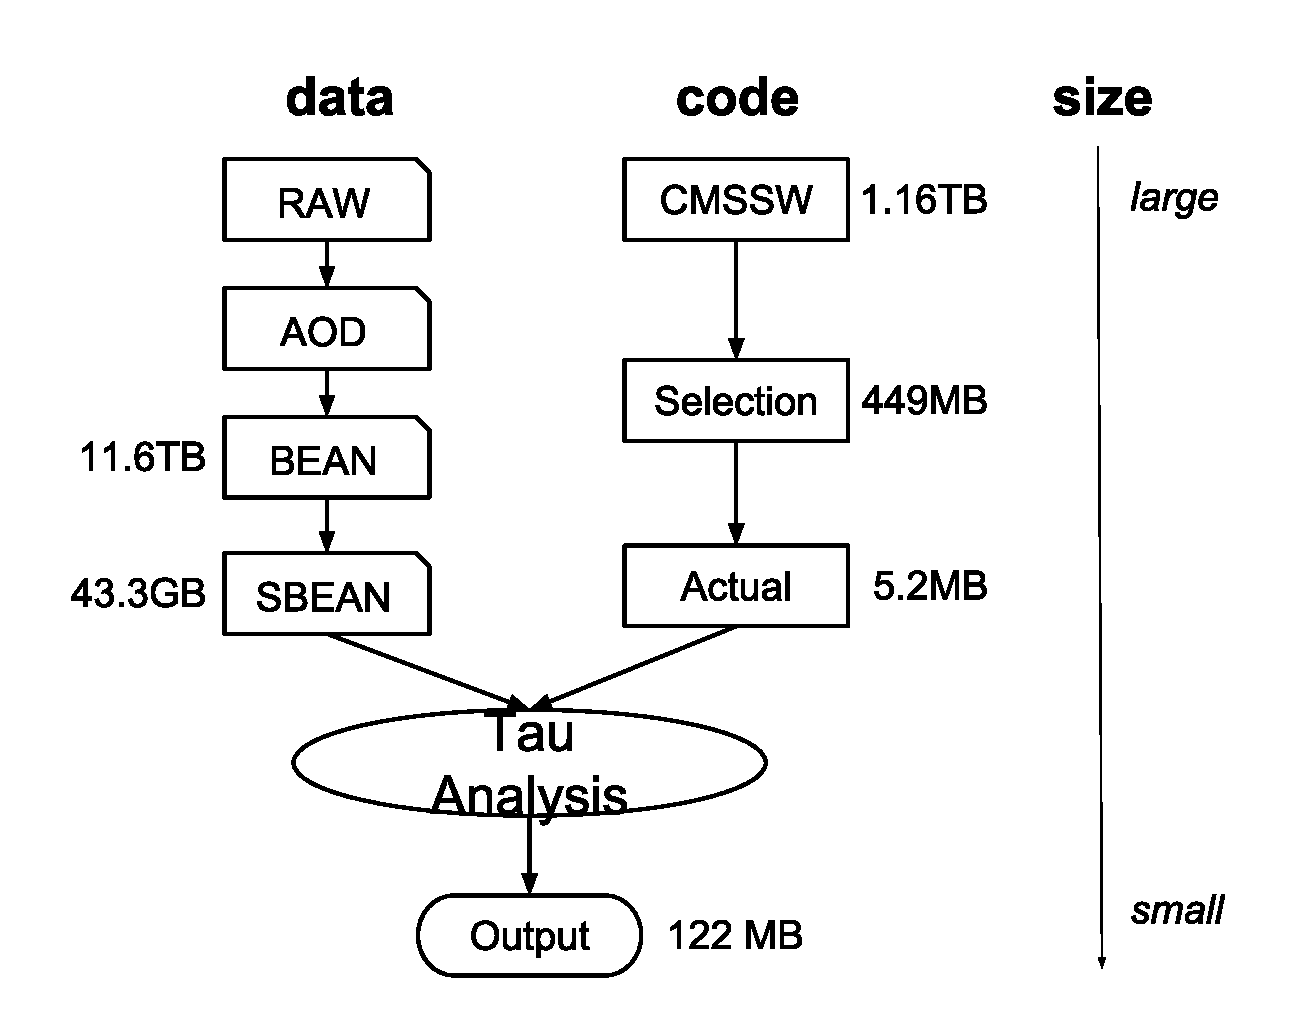
\includegraphics[width=.8\columnwidth]{data-code-size.eps}
\caption{Inputs to Tau Roast}
\label{fig:data-code-size}
\end{figure}

\begin{table}[t]
    \centering
    \small
    \begin{tabular}{|l|l|r|r|r|}
        \hline
        \bf Name & \bf Location & \bf Total & \bf Named & \bf Used \\ 
        \hline
        Ntuples data    & hdfs & 24TB & 43.3GB & 20GB \\ \hline
        CMSSW binaries     & local & 1.16TB & 448.3MB & 6.3MB\\ \hline
        Tau source       & git & 73.7MB & 73.7MB & 73.7MB \\ \hline
        PyYAML binaries    & http & 52MB & 51MB & 51MB \\ \hline
        .h file       & http & 41KB & 41KB & 41KB \\ \hline
        Misc commands & PanFS & 155TB & N/A  & 1.6MB \\ \hline
        Linux commands & localFS & 110GB &  N/A & 68.3MB \\ \hline     
        CVMFS & CVMFS & 7.4GB & N/A & 103MB \\ \hline
        NDCMS & optFS & 862GB & N/A & 53KB \\ \hline
        AFS & AFS &10.2GB & N/A & 34MB\\ \hline
        Total      &    & 181.1TB            & N/A & 21GB \\ \hline
    \end{tabular}
    \caption{Data and Code Used by Tau Roast}
    \label{table:size-original-real}
\end{table}

\section{Overview of Tau Analysis}

Within the ongoing investigation of the Higgs boson at the CMS
detector, part of the LHC at CERN, the Higgs production in association
with two top quarks allows to measure the Higgs coupling strength to
top quarks.  As the Higgs boson is to short-lived to be detected
itself, it has to be reconstructed from its decay products.

The application which is the study of this paper is called \emph{TauRoast}
It searches for cases where the the Higgs boson decays to two tau leptons.
The leptons are not observed directly, but by the particle showers
that they generate.  So, the analysis must search for detector
events that show a signature of decay products compatible with both hadronic tau and top decays.  Properties of such events are used to distinguish
the events of interest (Higgs decays) from all other events and
are also used in further statistical analysis.

Figure~\ref{fig:data-code-size} shows that both the code and data
that form \emph{TauRoast} are drawn from large repositories through
multiple steps of reduction.

{\bf Data Sources.}
The CMS collaboration provides analysis end-users with a pre-processed
and reduced data format, AOD, containing information for events, i.e.,
proton-proton collisions with a signature of interest, in the form of
reconstructed particles.  This format is based on the RAW output of
the CMS detector readout electronics and reconstructed world-wide.
Both real and simulated data are available for examination.

As AOD data are too large to be iteratively processed repetitively in
an physics analysis workflow, it is normally reduced further in
structural complexity and content.  For the analysis under
investigation here, this is a two-step process.  First, the AOD data
are processed at the Notre Dame working group cluster to BEAN events,
containing only trivial data containers packed in vectors.  This step
is time and CPU intensive and its output contains data of 11.6$\,$TB to be
analyzed by the tau analysis.
It is performed by a small custom code framework,
which is built on top of the CMS software stack, CMSSW,
and uses packages provided by several other special interest groups within CMS.
While the CMSSW framework is installed locally,
the various packages used are checked out from CVS,
and the BEAN framework is stored in git.
This is scheduled to change,
as the CMSSW distribution model switches to a virtual filesystem mounted via FUSE,
and special interest groups move their code to git.
The BEAN format, production code, and
data are shared within the analysis group looking at Higgs production
in association with top quarks, which is formed by groups from a few
American and European universities,
consisting of up to a few dozen contributors.

In the second step, which is the beginning of the actual tau analysis,
the data are reduced to variables relevant to the tau roast procedure, while
only events matching basic quality criteria are kept.  This results in
a dataset of 43.3$\,$GB.  Again, the Notre Dame CMS groups cluster
resources are used to perform this reduction and selection,
running highly customized software,
built on CMSSW and the BEAN framework,
but with output code written and maintained by a few people only.
Again, the code is stored in a git repository.

The final data analysis, investigated below, can be run as a single
process, and contains a stringent event selection to keep only high
quality candidate events for the underlying physical process (using
about 20$\,$MiB of space).  Quantities from the selected events can be
both plotted and used in multivariate analysis to determine the level
of expected signal in real data.
This package is written using the CMSSW build framework,
but only utilizes code from ROOT,
a particle physics toolkit underlying CMSSW,
and a few external python dependencies for convenience.
The latter have to be manually fetched and installed,
while the analysis program is built by CMSSW after being checked out of git.

{\bf Code Sources.} Like many scientific codes, the central algorithm
of \emph{TauRoast} is expressed in a relatively small amount of
custom code developed by the primary author.  But, the code cannot
run at all without making use of an enormous collection of software
dependencies.  Some of these dependencies are standard to operating
systems worldwide, some are standardized across the entire high-energy
physics field, some are particular to small collaborative groups,
and a few are very specific to a single researcher.

The largest of these repositories is the CMS Software Distribution (CMSSW),
a carefully-curated selection of software packages which is distributed
in binary form.  Historically, CMSSW was downloaded and installed on shared
filesystems within HPC centers.  In recent years, distribution has moved to
an on-demand delivery system known as CVMFS~\cite{cvmfs}.  The content
of CMSSW is managed very carefully by a centralized team whose main goal
is to ensure that the current version of the software operates correctly
on the operating systems and architectures currently in use.  However,
preservation per se is not an objective of the group, and so there is
no guarantee that old versions of CMSSW operate in new environments,
or vice versa. 

\emph{TauRoast} was provided to us in the form of an
email which described, in prose, how to obtain the source,
build the program, and run it correctly on one specific
machine at Notre Dame, with no particularly guarantee that
it will run anywhere else in the world.
Although this starting point may seem extreme, it is
perfectly natural for collaborators to share configurations
with each other in this form, and to rely on the presence
of a working environment with appropriate dependencies already
installed.

The authors played the role of curators, whose job it is to prepare the application for permanent archival by determining and packaging the dependencies.

\subsection{Workflow of Matthias's Example}

The workflow of Matthias's exmaple can be divided into eight procedures.

(a) Declare environment variables

(b) Obtain software from CMSSW

(c) Obtain software from Git

(d) Obtain software from some public HTTP web links

(e) Obtain software from one private home page

(f) Build software enviroment using SCRAM and Python

(g) Install grid control, obtain CMS data from grid and store the data into HDFS mounted as one local file system.

(h) Actual data analysis.

\subsection{Key Observations of the Example}

\subsubsection{Complexity of Data and Software Dependencies}

\begin{figure}[t]
\centering
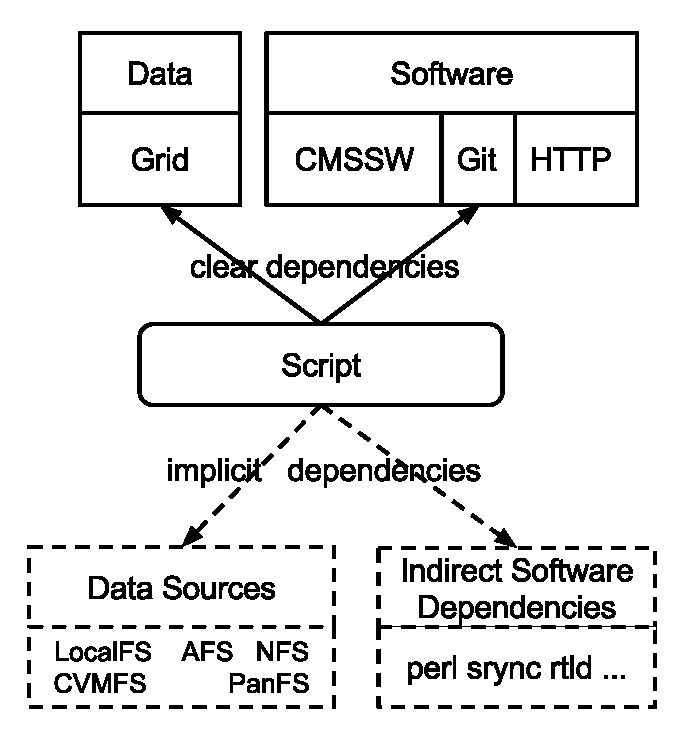
\includegraphics[width=.8\columnwidth]{dependencies.eps}
\caption{Dependencies}
\label{fig:dependencies}
\end{figure}

Figure~\ref{fig:dependencies} illustrates all the dependencies
involved in the program, which can be divided into two categories: clear
dependencies and implicit dependencies. Clear dependencies include scientific data
dependencies and direct software dependencies which can be extracted directly
from the analysis program. The scientific data of this example comes from the Grid. Direct software dependencies include CMSSW, Git, HTTP and one personal home page. 

Implicit dependencies include indirect software
dependencies which is necessary for the successful execution of direct software
dependencies and other implicit dependencies. For example, we know Git is one
direct software dependency from the analysis program, which further depends on
perl, python, rsync, openssh-clients and other packages. The analysis program
accesses one file called File1, which is one symbolic link file further referring to
another file named File2.
The implicit dependencies also refers to some files under {\tt /pscratch}, which is a local mount point of one PanFS with the size of 206TB.
And more importantly, the successful execution of this program greatly depends on the underlying OS and hardware platform.

\subsubsection{Size of Data and Software Dependencies}
The size of data and software dependencies is astonishing.
The size of BEAN is 11.6TB, which is too large to be analyzed directly by the tau roast program. After one preprocessing which only collects the events matching basic quality criteria, the data size is still very large, 43.3GB. 

The size of software from each source is shown in Table~\ref{table:software-source-size}.

\subsubsection{Complexity of the Program}
Complex data and software dependencies, complex environment building process, the large size of data and software involved in the tau roast program, together with the access authority problem, determine the complexity of the program. 
In order to obtain the experimental data from the Grid, the author needs to install and config grid-control software. 
The access authority of the Grid is also necessary for the data acquisition.
The software acquisition from CMSSW, Git and HTTP and environment building process is time-consuming. The execution time of actual data analysis is about 30 minutes. However, the software acquisition and environment building time, excluding data acquisition time, is about 30 minutes, which is very close to the execution time of actual data analysis. If the acquisition of experimental data is considered, actual data analysis only occupies one small percentage of the whole time consumption.
The size of data and software dependencies further complicate the program.

\subsubsection{Really Used Data and Software Size} 

Even if the orginal data size referred by the program is astonishing, the size
of really used data and software is greatly smaller.
Figure~\ref{fig:data-code-size} illustrates the inputs of the tau roast program.
After the TauAnalysis procedure, the data size of Ntuples is 43.3GB, however, the atual size of really used
data in the program is 20GB.  The same trend occurs to the size of software and
other dependencies. The size of CMSSW repository is 1.16TB, the size of
packages checked out from CMSSW is 449MB, and the size of actually used CMSSW
files is only 5.2MB. 
The total size of PanFS mounted as {\tt /pscratch is 206TB}, however, the really used data from {\tt /pscratch} is only 119MB.
We compared the original size and actually used size of data and software in Table~\ref{table:size-original-real}.

\subsubsection{Stability of Dependencies}

The program involves obtaining software from the home page of another graduate
student from University of Notre Dame. However, the maintenance of this
home page will terminate after the graduation of the student.
The stability of each dependency must be evaluated to ensure the program can be 
repeated by others.

The stability of the Grid is relatively higher. However, the
public web resources and personal home page is not stable. Too many factors
like the termination of one web site, the graduation of the home page's author,
would result in the failure of resource access. CMSSW, which seems to be
stable, in fact, also involves stability problems. CMSSW provides different
collections of accessible versions to different architectures. Transformation
from one architecture to another may result in the failure of accessing one
certain CMSSW version. At the beginning of our reseach, cvs supported
anonymous access of CMSSW outside of CERN. However, this anonymous access has
been cancelled now.

\begin{table}
    \centering
    \begin{tabular}{|l|}
        \hline
        {\bf Version 1: Email}\\ \hline
        1. Create a CMS release,\\
            \hspace{9pt} e.g. {\tt cmsrel CMSSW\_5\_3\_11\_patch3} \\
        2. Install the BEAN packages as the instructions: \\
            \hspace{9pt} {\tt \url{https://github.com/cms-ttH/BEAN/blob/...}}\\
        3. Install grid-control: \\ 
            \hspace{9pt} {\tt svn co \url{https://ekptrac.physik.uni-ka/...}} \\
        4. INstall the TauAnalysis package: \\
           \hspace{9pt} {\tt git clone \url{https://github.com/matz-e/...}} \\
           \hspace{9pt} {\tt scram b -j32} \\
        5. Fix grid\_control.cfg and run it. \\
        6. Perform the actual tau roast program. \\ 
        \hline
        {\bf Version 2: Script}\\ \hline
        {\tt set CMSSW\_BASE = (CMSSW\_5\_3\_11\_patch3)} \\
        {\tt cmsrel \$HOME/\$CMSSW\_BASE} \\
        {\tt cvs co -r V03-09-23 PhysicsTools/PatUtils} \\
        {\tt git clone \url{https://github.com/cms-ttH/BEAN.git}} \\
        {\tt wget -r \url{http://nd.edu/~abrinke1/...}} \\
        {\tt scram b -j32} \\
        {\tt wget \url{http://pyyaml.org/download/pyyaml/PyYAML...}}\\
        \#the experiment data is from HDFS \\
        {\tt cd \$HOME/\$CMSSW\_BASE/src/PyYAML-3.10}\\
        {\tt cmsenv}\\
        {\tt python setup.py install --user} \\
        {\tt scripts/roaster data/generic\_ttl.yaml} \\ 
        \hline
        {\bf version 3: Formulated Script} \\ \hline
        {\tt set CMSSW\_BASE = (CMSSW\_5\_3\_11\_patch3)} \\
        {\tt set {\bf GIT} = (\url{https://github.com})} \\
        {\tt set {\bf PYYAML} = (\url{http://pyyaml.org})} \\
        {\tt set {\bf ND} = (\url{http://nd.edu})} \\
        {\tt cmsrel \$HOME/\$CMSSW\_BASE} \\
        {\tt cvs co -r V03-09-23 PhysicsTools/PatUtils} \\
        {\tt git clone \${\bf GIT}/cms-ttH/BEAN.git} \\
        {\tt wget -r \${\bf ND}\url{/~abrinke1/ElectronEffectiveArea.h}} \\
        {\tt scram b -j32} \\
        {\tt wget \${\bf PYYAML}/download/pyyaml/PyYAML...}\\
        \#the experiment data is from HDFS \\
        {\tt cd \$HOME/\$CMSSW\_BASE/src/PyYAML-3.10}\\
        {\tt cmsenv}\\
        {\tt python setup.py install --user} \\
        {\tt scripts/roaster data/generic\_ttl.yaml} \\ 
        \hline
       {\bf Version 4: Fine-Grained Toolkit}\\ \hline
        {\tt set CMSSW\_BASE = (CMSSW\_5\_3\_11\_patch3)} \\
        {\tt set {\bf GIT} = (\url{https://github.com})} \\
        {\tt set {\bf PYYAML} = (\url{http://pyyaml.org})} \\
        {\tt set {\bf ND} = (\url{http://nd.edu})} \\
        {\tt cmsrel \$HOME/\$CMSSW\_BASE} \\
        {\tt cvs co -r V03-09-23 PhysicsTools/PatUtils} \\
        {\tt git clone \${\bf GIT}/cms-ttH/BEAN.git} \\
        {\tt wget -r \${\bf ND}\url{/~abrinke1/ElectronEffectiveArea.h}} \\
        {\tt scram b -j32} \\
        {\tt wget \${\bf PYYAML}/download/pyyaml/PyYAML...}\\
        \#the experiment data is from HDFS \\
        {\tt cd \$HOME/\$CMSSW\_BASE/src/PyYAML-3.10}\\
        {\tt cmsenv}\\
        {\tt python setup.py install --user} \\
        {\tt scripts/roaster data/generic\_ttl.yaml} \\ 
        \hline
    \end{tabular}
    \caption{Scripts of each Solution}
    \label{table:scripts}
\end{table}

\begin{figure*}
\centering
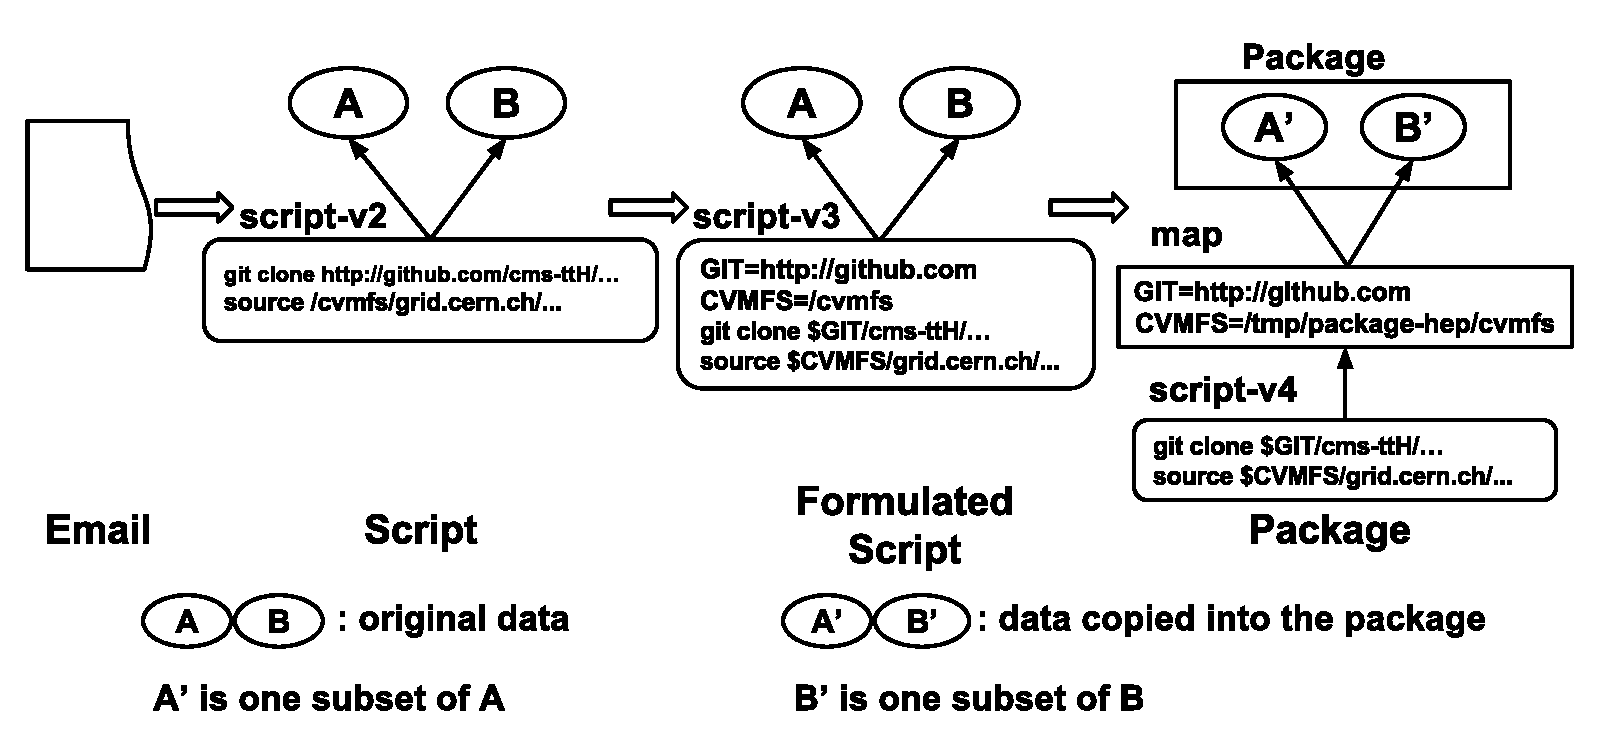
\includegraphics[width=1.6\columnwidth]{version-evolution.eps}
\caption{Version Evolution}
\label{fig:version-evolution}
\end{figure*}

\section{Preservation Strategies}

Figure~\ref{fig:version-evolution} illustrates the evolution history of different preservation strategies.

\subsection{Solution 1: Email}

In order to repeat Matthais's example, the new user consulted the original
author by email about the necessary work for the experiment. In response,
Matthias introduced the general workflow of his tau roast program through one long
email including notes, linux shell commands, web links. The Version 1 of
Table~\ref{table:scripts} illstrates his email.

However, this solution to repeat one experiment has three potential drawbacks.
Firstly, the experience of repeating one tau roast program through emails is
chaotic. You need to constantly jump around multiple web links. There are overlap
between the content of the email and the content of web links, which needs the
new user to merge them. Multiple communication through emails is necessary to
ensure the successful reproduction of the whole analysis. For example, the original
email refers to one environment variable called CMSSW\_base without clear
declaration, the new user needs to send one email to the original writer to
obtain its accurate value. Secondly, the necessary procedures to repeat the
experiment, including software acquisition from different sources, is complex
for the new user. In Matthias's example, the sources of software includes
CMSSW, Git, HTTP. The access of CMSSW requires the new user to be an authorized
user of CMSSW. What's more, some parts of the workflow are unrepeatable. The
third step of this experiment requires the new user to own the access authority
of the Grid. 

Implication: Directly repeating the experiment using the workflow description and results provided by the original author is complex and difficult. Some extra work must be done to make the reproduction process easier.

\subsection{Solution 2: Script}
One possible solution for the access authority problem of grid data is to grant the new user the authority to access gird data directly. Another possible solution is let the new user directly operate on the machine the original author used. As for the complexity of jumping between multiple web links, people may suggest that letting the original author generate one clear script including all the contents from different web links.

To test out these possible solutions, we integrate the content of all the notes, commands and web links involved in the emails into one neat, complete shell script, which begins with the definition of environment variables, software acquisition from CMSSW, Git and other web resources, and software installation, ends with the execution of the actual analysis program. Version 2 of Table~\ref{table:scripts} illstrates the merged script. As for the data acquisition from the Grid, we directly use the local copy in HDFS to avoid requiring the new user to obtain a grid certification.


%*****hmeng-doult: the size of hadoop need to reconsidered. how to correctly illustrate the data size of this example?

Because the script includes all the necessary procedures for the reproduction
of one analysis program, the readability and friendliness of this solution is
higher than that of the email format. 


\subsection{Solution 3: Formulated Script}
%%

The script can reduce the complexity of repeating one experiment through the integration of all the necessary procedures. However, the data and software dependencies are still randomly distributed across the whole script, which requires one complete scan of the script to obtain the  dependency list. 

To further separate the data and software dependencies from the actual analysis
script, we formulate the Version 2 of Table~\ref{table:scripts}  into one new version, as shown in
the Version 3 of Table~\ref{table:scripts}. Each new environment variable at the beginning part of
the script is corresponding to one dependency. All the following access to data
or software dependency will refer to its corresponding environment variable.
All the environment variables of dependencies form one map, which maintains the
target address of each dependency.

This script style may function as one new guideline to the original author of one experiment, which expresses the dependencies more clearly and expedites the preparation process to 
repeat one experiment. The introduction of the map file also reduces the workload of changing one dependency. For example, if we want to utilize one new git package to analyze the same dataset, only the change of environment variable corresponding to the original git package is necessary. Without the map file, the whole script needs to be scanned to figure out and replace all the references of the original git package.

However, each execution of the script
will involve the acquisition of software from different sources and the
building of software environment. As for accessing grid data, using the data
copy stored in the machine where Matthias executed the experiment requires the
new user to have the authority to access the machine, which complicates the
management of the original machine, even is impossible if the original machine
executes rigid user access control. Granting everyone who wants to repeat the
analysis the access authority for grid is unacceptable to system administrator. 

Implication: All the data and software involved in the experiment should be
provided to the new user in the format of one self-contained package so that
the new user can avoid complex data and software acquisition and software
environment building process. In addition, the requirements of the underlying
OS and hardware should also be provided to the new user.

\subsection{Solution 4: Package}
The difficulty of data access authority acquisition enforces us to find out one
solution, in which the reproduction of the original analysis can be done
without any external dependency. That is, one independent and self-contained
package containing all the data and software dependencies is necessary. 

Someone may suggest that it should be the responsibility of the original author
to generate the required package. However, letting the original author provide
the package which can be used by others to repeat the original experiment is
unrealistic. One reason is that figuring out the underlying dependencies of
each software is complex and time-consumpting and even impossible for the
original author. In this experiment, the machine used for the experiment is one
public machine of physics department, and Matthias is one common user without
root authority. The underlying OS and supporting softwares are installed and
maintained by the IT department of the university. On the other hand, the
architecture design of the required package including all the data and software
dependencies is not under the research field of physists.

To generate one self-contained and independent package for one experiment, all
the clear and implicit dependencies must be figured out firstly. The map file
of Solution 3 can provide clear data and software dependencies. As for the
implicit dependencies, directly preserving the whole OS together with the data
stored on the disk of the original machine or the data from other filesystems
mounted as local filesystems, such as HDFS and PanFS,  is not feasible. One
efficient mechanism which can figure out the really used parts of all these
filesystems is necessary. The requirements of the underlying OS and hardware
architecture can be easily found with system tools such as uname or
lsb\_release.

Then one new package including all the data and software dependencies can be generated and published. 
One packaging utility is necessary for the original author to generate the package. 
To multiplex the common data which is involved in different experiments, such as OS images and common software library, the data of different packages will be rearranged and categorized in the archive.
One description file, which includes the experiment aim, dependency list,  package size and relevant information, will be generated for each package.

\begin{figure}
\centering
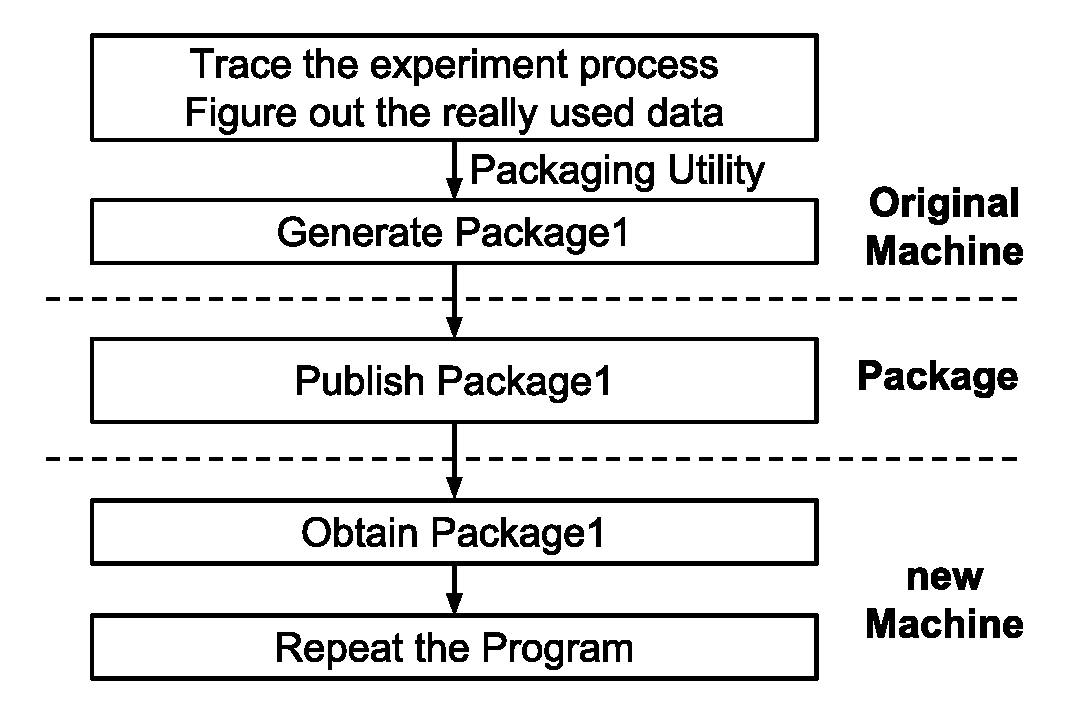
\epsfig{file=solution3.eps, height=2in, width=3in}
\caption{Relationship of Roles}
\label{fig:solution3}
\end{figure}

The relationship of different roles involved in the experiment preservation and
reproduction is shown in Figure~\ref{fig:solution3}.  The original author is
responsible for generating one package based on the successful execution
with the help of the packaging utility. Then the package, together with
its map file and description file will be uploaded into the archive. When
another scholar wants to repeat the experiment, one copy of the package and its
corresponding map file will be downloaded into the new machine.

\begin{table}
    \centering
    \begin{tabular}{|l|l|}
        \hline
        Archive Path & Service Description \\ \hline
        {\tt /archive/OS/path} & OS Image \\ \hline
        {\tt /archive/software/path} & Common Software Library \\ \hline
        {\tt /archive/CMSSW/path} & CMS Software Library \\ \hline
        {\tt /archive/git/path} & Git Software Library \\ \hline
        {\tt /archive/http/path} & http resources \\ \hline
        {\tt /archive/experiment/path} & experiment private files \\ \hline
        {\tt /archive/grid-data/path} & data from the Grid \\ \hline
    \end{tabular}
    \caption{Structure Organization of the Archive}
    \label{table:archive-map}
\end{table}

Table~\ref{table:archive-map} illustrates the structure of the remote archive.
{\tt /archive/OS} includes the images of different Operating Systems.
{\tt /archive/software} integrates all the commonly used software, such as git,
python, perl. The archive also organizes the data from CMSSW, Git, HTTP and the
Grid. {\tt /archive/experiment} includes the all the experiments submitted into the
archive. The private files and description files of each experiment will be
organized together.

The Version 4 of Table~\ref{table:scripts} illustrates the script used in
Solution 4, which is the same as the one used in Solution 3. 
However, one map file is necessary for the relocation of the data access targets, as
show in Figure~\ref{fig:version-evolution}. 
The map file redirects the git access path into {\tt /archive/git} from the original path (\path{http://github.com}) referred in the script.
This design decouples the experiment script and the actual data access targets, which minimizes the impact of the evolution of different data dependencies
and ensures the transparent access.
The modification of the archive only introduces the minimal changes of the map file.

The archive supports two different data preservation model: Internal and External. Internal method will preserve the data in the archive. External method refuses to preserve the content of data, but only preserve the reference to the actual storage place of data. For example, the size of experiment data from the Grid is extremely large, and storing the same data in the archive is time-consuming and space-consuming. Through External method, the archive only preserves one reference to the data inside the remote Grid.

This solution tries to create one self-contained and independent package for each experiment and integrate different packages for different experiments into one archive to multiplex common data. One packaging utility  will be provided to help the original author to generate the package. The archive can maintain the experiment dependencies through Internal or External method. The archive itself will be responsible for the data maintenance and relevant authority access problem. All the new user can repeat one experiment through the interaction with the archive.

\section{One Implemention of Fine-Grained Toolkit Using Parrot}
\subsection{Working principle of Packaging Utility} 

Parrot is a virtual filesystem access tool which attaching existing programs to
a variety of remote {\tt I/O} systems including http, ftp, gridftp, irods, HDFS,
xrootd, grow and chirp. It traps all system calls of one program through ptrace
debugging interface, and replaces them with remote {\tt I/O} operations as desired.
Through executing one program under Parrot, all the paths of files involved in
this program can be recorded.  

With the help of Parrot, one packaging utility which generates one independent
package for one program to make the reproduction of the program convenient can
be deployed. The starting point of the packaging utility is one successful execution
sandbox (the data from grid has been preserved in HDFS and the software from
CMSSW, Git and HTTP has been on the local machine.). We re-execute the actual
data analysis code under Parrot and get the name list of all the files actually
accessed during the execution process of the actual data analysis. Then,
according to the file name list, one package containing all the necessary data
and software for one analysis program is generated. Next time, when another
scholar wants to repeat the program, he only needs to obtain the package and
directly execute the actual analysis program inside the package.

\begin{table}
    \centering
    \begin{tabular}{|l|}
        \hline
        {\tt set CMSSW\_BASE = (CMSSW\_5\_3\_11\_patch3)} \\
        {\tt cd \$HOME/\$CMSSW\_BASE/src/PyYAML-3.10}\\
        {\tt cmsenv} \\
        {\tt python setup.py install --user} \\
        {\tt cd \$HOME/\$CMSSW\_BASE/src/ttH/TauRoast}\\
        {\tt scripts/roaster data/generic\_ttl.yaml} \\
        \hline
    \end{tabular}
    \caption{Script of Fine-Grained Toolkit using Parrot}
    \label{table:parrot-script}
\end{table}

The shell script of the Solution 2 is simplified into one new version, which
only contains the necessary environment variables and the
actual analysis command. Table~\ref{table:parrot-script} illustrates
the simplified script.

\subsection{Workflow of Packaging Utility}
\begin{figure*}
\centering
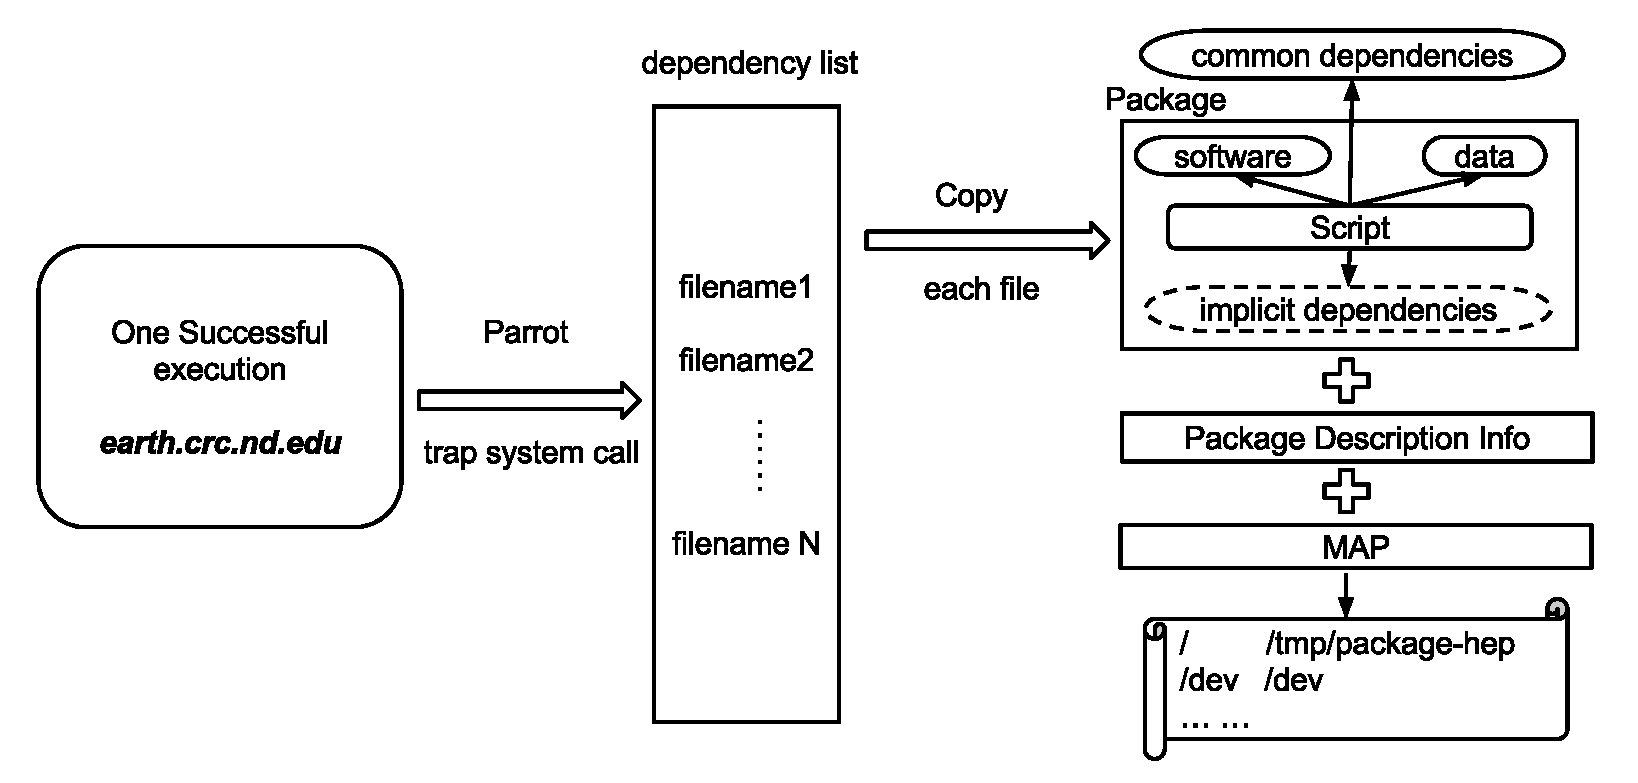
\epsfig{file=workflow-parrot.eps, height=4in, width=6.5in}
\caption{Workflow of Solution 4}
\label{fig:workflow-parrot}
\end{figure*}

Figure~\ref{fig:workflow-parrot} illustrates the workflow of this solution.

The workflow of generating one package for one analysis program is as follows.

(1) execute one analysis program under Parrot and obtain filename list (L1) of it

Parrot is one virtual file system that can support user access to multiple underlying file systems. Parrot traps each system call involved in the process of data access, figures out the type of file system and redirects it into corresponding operations to the accessed file system. During this process, each accessed file is recorded into one file with the access type of it, such as open, stat, read and write.

The command used to generate the file name list is as follows. The {\tt -L} parameter refers to the path of the file containing all the accessed file name of the experiment.

{\tt parrot\_run -L namelist /bin/tcsh script\_v4.sh}

The original ouput of this command is one namelist file with the size of 6.6MB
and 132,058 lines, each of which corresponds to one one accessed file of the
program. We noticed that some items appeared multiple times. To reduce the
packaging time, de-duplication and sorting techoniques are used for the
namelist file, generating one smaller file with the size of 3.2MB and 67,178 lines.

(2) generate one package containing the files of L1 

The packaging utility iterates each filename inside L1 and copies it into the
target package. After finishing the packaging process, the target package
together with its description information, and one map file, which redirects
the access of files from different file systems into the files inside the target package, will be
provided to users. The packaging process also runs within Parrot environment to
access data from different file systems.

\begin{figure}
\centering

\epsfig{file=package-info.eps, height=1.2in, width=2.5in}
\caption{Package Description Infomation}
\label{fig:package-info}
\end{figure}
The command used to generate the package containing all the files of L1 is as follows. 
{\tt package-utility.sh} is a bash script which iterates each line of L1 and
determines the behavior according to the file type (common files, directories,
linked files) and the system call type.
The package description information is shown in Figure~\ref{fig:package-info}.

{\tt parrot\_run /bin/bash package-utility.sh -L namelist}

%*****lack: file content + metadata; only file metadata; different process
%solutions
Each file inside L1 is copied into the package, the final path of the file
becomes the path of the package, followed by the original file path. In this
program, the path of the package is {\tt /tmp/package-hep}, so the final path of one
file with the original path path1 is {\tt /tmp/package-hep/path1}.

To ensure the successful reproduction, the filesystem structure of the original
execution environment should be preserved as completely as possible. However,
attempting to copy the whole content of one directory or one file is
space-consuming and time-consuming, because the original program may only
access the metadata of one file with the size of 200GB. Our solution is to
determine the copy degree of one directory or one common file according to the
system call type for its path.

The map relationship between the file access path used in the actual analysis
program and the actual file location used during the reproduction process is
kept inside the map file. The structure of the map file is shown in Table~\ref{table:map-file}.

\begin{table}
    \centering
    \begin{tabular}{|l|l|}
    \hline
    Path used in Program & Actual Location \\ \hline
    {\tt /} & {\tt /tmp/package-hep} \\ \hline
    {\tt /tmp/package-hep} & {\tt /tmp/package-hep} \\ \hline
    {\tt /dev} & {\tt /dev} \\ \hline
    {\tt /misc} & {\tt /misc}\\ \hline
    {\tt /net} & {\tt /net}\\ \hline
    {\tt /proc} & {\tt /proc}\\ \hline
    {\tt /sys} & {\tt /sys}\\ \hline
    {\tt /var} & {\tt /var}\\ \hline
    {\tt /selinux} & {\tt /selinux}\\ \hline
    \end{tabular}
    \caption{Structure of Map File}
    \label{table:map-file}
\end{table}

%*****lack: re-execute process: re-execution process will redirect all the data access into the package except for data under proc sys dev selinux
(3) rerun the analysis program using the package

When another scholar wants to repeat one analysis program, the accessed data
field is limited into the target package with the help of the map file 
generated in step 2. 

Command:

{\tt parrot\_run -m /tmp/mountlist /bin/tcsh script\_v4.sh}

\subsection{Structure of Map File} 

The map file of one package supports pattern matching semantics,
which greatly reduces the scale of the map file and improves the efficiency of file path redirection. 
For example,
one item inside the map file is {\tt /dir1 /package-dir1} means that the access to each file and
subdirectory under {\tt /dir1} will be redirected into {\tt /package-dir1}.
If the semantics of the map file do not support pattern matching, the size of the map file will become astonishing. 
{\tt /dir1} may contain thousands of files, which will generates thousands of map items and will take more time to redirect file paths.

During the packaging process, we noticed
that it is impossible to copy the files under certain directories.
For example, during namelist acquisition process, three special files under {\tt /dev} directory were recorded into the namelist: tty, null and urandom, which are used for input and output.
We tried to copy these files into the new package, but the packaging utility halted.
We also noticed that copying the files under directories like {\tt /proc} is
meaningless. Because the process id of one program is random and depends on the
current allocation of process ID. 

As for these two file categories, letting
the program directly utilize the files on the machine, where the new user
repeats the program, is a better choice. The semantics is implemented by
setting the target path of one file equal to the origin file path inside the
map file. For example, {\tt /dev /dev} means that when the program needs to access
files under {\tt /dev} directory, it will directly use the file under {\tt /dev}, which is
independent from the namespace of the package. This semantics also makes the
reference of files outside the package possible. If the new user wants to
expand the analysis of one program to his own data with the path of {\tt /A}, he can add the analysis
code into the analysis script and add one item {\tt /A /A} into the map file.


\subsection{Discussion of Solution 4} 

Under Solution 4, the reproduction of one analysis program becomes easier.
Rethink Matthias's example, the reproduction of it only needs
the necessary environment variables, the actual analysis command
and the package. If different scholars want to repeat one analysis program,
what they need to do is to obtain the package and rerun the actual analysis
program. Under Solution 2, each scholar needs to get the necessary data and
software, and then prepare software environment. 

%here is the new content-hmeng
The starting point of Solution 4 is one successful execution sandbox on the original machine. 
Parrot traps all the system calls and copies each accessed file (except for common dependencies) into one package.
The necessary scientific data will be copied into the target package.
The software dependencies can be divided into two categories: clear dependencies, which can be observed directly through reading the analysis script and implicit dependencies,
which can not be obtained through reading the analysis script. 
Parrot can obtain every dependency through trapping each system call.
Strictly speaking, the software concept and the scientific data concept are lost in Solution 4, because
the granularity of parrot is file.
The same thing happens to networked resources.
Packaging utlity maintains one list of common dependencies and first judges whether the file belongs to this list before trying to copy one file into the package.
As for the computing environment, Solution 4 notices the new user through the description information at the beginning of the script.
%the following subsection belongs to the "discussion of data and software
%preservation" section

\begin{table*}
    \centering
    \begin{tabular}{|l|r|r|r|}
        \hline
        Solution ID & Data Resources & Software Resources & Operation Manual \\ \hline
        Solution 1& grid & CMSSW Git HTTP & email \\ \hline
        Solution 2 and 3& local (HDFS) & CMSSW Git HTTP & shell script \\ \hline
        Solution 4& package & package & shell script + packaging utility \\ \hline
    \end{tabular}
    \caption{The relationship of different solutions}
    \label{table:relationship}
\end{table*}

%The fourth solution should be based on the third solution. during the packaging process, packaging utility first checks whether the file has been inside the target package, (if exists, whether it is the latest version). only if the file does not exist in the target package or the file in the target package is not the latest version, the packaging utility copies the file into the target package.

%*****hmeng-doubt: potential risk: different analysis programs share some common file names, but with different file contents. we should analyze the possibility of conflict: data.

%*****hmeng-doubt: in the fourth version, let user to mark whether they change the data and software. if changed, one new package is generated to avoid data overlap and pollution. otherwise, directly starts packaging process based on the current target package. 
\section{Evaluation}
\subsection{Relationship of Different Solutions}
The relationship of these three solutions to repeat one program is shown in Table~\ref{table:relationship}. The aim is to make it easier to repeat one program through making the data and software preparation easier.

\subsection{Evaluation of Solution 2}
The breakdown of execution time of Solution 2 is shown in Table~\ref{table:time-2nd}. About half of the total execution time is consumed to prepare relevant software environment. The cvs command is forked to check out 23 packages from CMSSW and three git repositories are cloned.

\begin{table}
    \centering
    \begin{tabular}{|l|r|r|}
    \hline
    Sub-Task & Time & Percentage \\ \hline
    Software acquisition from CMSSW & 7min 24s & 21.44\% \\ \hline
    Software acquisition from Git & 9s & 0.43\% \\ \hline
    Software acquisition from Wget & 38s & 1.83\% \\ \hline
    Environment Build - SCRAM & 5min 48s & 16.80\% \\ \hline
    Environment Build - Python & 1s & 0.05\% \\ \hline
    Data analysis & 20min 31s & 59.44\% \\ \hline
    Total & 34min 31s & 100.00\% \\ \hline
    \end{tabular}
    \caption{Breakdown of Execution Time of Solution 2}
    \label{table:time-2nd}
\end{table}

The size of data and software from each category is shown in table~\ref{table:datasize-2nd}.

\begin{table}
    \centering
    \begin{tabular}{|l|r|}
    \hline
    Data Category & Data Size \\ \hline
    Software from CMSSW & 448.3MB \\ \hline
    Software from Git & 73.7MB \\ \hline
    Software from Wget & 52MB \\ \hline
    HDFS & 43.3GB \\ \hline
    Total & 43.86GB \\ \hline
    \end{tabular}
    \caption{Data Size of Solution 2}
    \label{table:datasize-2nd}
\end{table}

\subsection{Evaluation of Solution 4}
The breakdown of execution time of the Solution 4 is illustrated in Table~\ref{table:time-3rd}. The time used to obtain file namelist and generate P1 is greatly longer than the execution time within the new package. however, the time consumption of file namelist acquisition and package generation is one-time. That is, once the package is generated, many users can directly obtain the package and repeat the experiment separately. 

\begin{table}
    \centering
    \begin{tabular}{|l|r|}
    \hline
    Sub-Task & Time \\ \hline
    Obtain file namelist & 28min 23s \\ \hline
    Generate P1 & 85min 51s \\ \hline
    Re-run the program within P1 & 13min 4s \\ \hline
    \end{tabular}
    \caption{Time Breakdown of Solution 4}
    \label{table:time-3rd}
\end{table}

The data size of Solution 4 is shown in Table~\ref{table:datasize-3rd}. The
data categories is more complex than our imagination. Except the data stored in
Hadoop and the necessary set of software, files from {\tt /pscratch, /sbin, /lib} and other
paths are also necessary for the reproduction of the program.

\begin{table}
    \centering
    \begin{tabular}{|l|l|r|}
    \hline
    Data Category &Location & Data Size \\ \hline
    HDFS & hadoop &20GB \\ \hline
    PanFS & opt & 1.6MB \\ \hline
    CVMFS & cvmfs &103MB \\ \hline 
    NDCMS & opt &53KB \\ \hline
    AFS & afs &34MB \\ \hline
    Local FS& bin etc lib lib64 sbin tmp usr&68.3MB \\ \hline
    Total & &21GB \\ \hline
    \end{tabular}
    \caption{Data Size of Solution 4}
    \label{table:datasize-3rd}
\end{table}    

\subsection{ Data size Comparison of Solution 2 and 4}

The packaging utility checks the system call of each file within the namelist,
and maintains the minimum dataset, which makes the size of the final package 
as small as possible. The total size of Hadoop under Solution 2 is astonishing,
while the size of Hadoop under the package is decreased to 20GB. The same trend
applies to the size of CMSSW\_5\_3\_11\_patch3. Because the packaging utility
tries to construct one independent and self-contained package, necessary files
from {\tt /sbin, /lib} and other directories are also copied into the package and
denoted as "Other data for Package" in Table~\ref{table:datasize-2nd3rd}.

\begin{table}
    \centering
    \begin{tabular}{|l|r|r|}
    \hline
     Data Category & Data Size & Data Size \\
    & Solution 2 & Solution 4\\ \hline
    HDFS & 43.3GB & 20GB \\ \hline
    PanFS & 155TB & 1.6MB \\ \hline
    CVMFS & 7.4GB &103MB \\ \hline
    NDCMS & 862GB &53KB \\ \hline
    AFS & 10.2GB &34MB \\ \hline
    Local FS& 110GB&68.3MB \\ \hline
    Total & 156TB &21GB \\ \hline
    \end{tabular}
    \caption{Data Size Comparison beweeen Solution 2 and 4}
    \label{table:datasize-2nd3rd}
\end{table}

\subsection{Execution Time Comparison of Solution 2 and 4}

Table~\ref{table:time-2nd3rd} shows the execution time comparison between
Solution 2 and 3. The time consumption of the reproduction of one program from
different scholars kept the same under Solution 2, including software and data
preparation. However, under Solution 4, the data and software preparation is
one-time. The following reproduction of the same program only needs to obtain
one copy of the package and execute the actual experimental analysis directly.
Data is obtained through accessing Hadoop Distributed File System in Solution 2, but is copied into the package in Solution 4. This localization of data speeds up the data analysis process, resulting the actual analysis time reducing from 31 minutes to 13 minutes.

\begin{table}
    \centering
    \begin{tabular}{|l|r|r|}
    \hline
    Task Category & Execution Time & Execution Time \\
    & Solution 2 & Solution 4\\ \hline
    Software Acquisition & 8min 11s & N/A \\ \hline
    Environment Building & 5min 49s  & 3s \\ \hline
    Obtain file namelist & N/A & 28min 23s \\ \hline
    Generate the package & N/A & 85min 51s \\ \hline
    Actual Analysis & 20min 31s & 13min 4s \\ \hline
    \end{tabular}
    \caption{Execution Time Comparison between Solution 2 and 4}
    \label{table:time-2nd3rd}
\end{table}    

%*****hmeng-doubt:Another reason for the packaging utility is that not all the data and software generated by the second version script is used during the the actual data analysis. The packaging utility can help us find out the optimal subset of data and software involved in one actual data analysis. 
%*****hmeng-doubt: this point is not the motivation. but one achievement comes together. out of imagination.
\section{Discussion of Data and Software Preservation}
\subsection{Preservation Integration of Multiple Programs}
The Solution 4 can work well for the preservation and reproduction of one single program. However, different experimenters may execute different analysis programs on the same dataset using the same or overlapping sets of software. Generating one new package for each analysis program from scratch is time-consuming and space-consuming, which makes one data and software preservation mechanism, that can integrate the preservation requirements of different analysis programs, become necessary. 

\begin{figure}
\centering
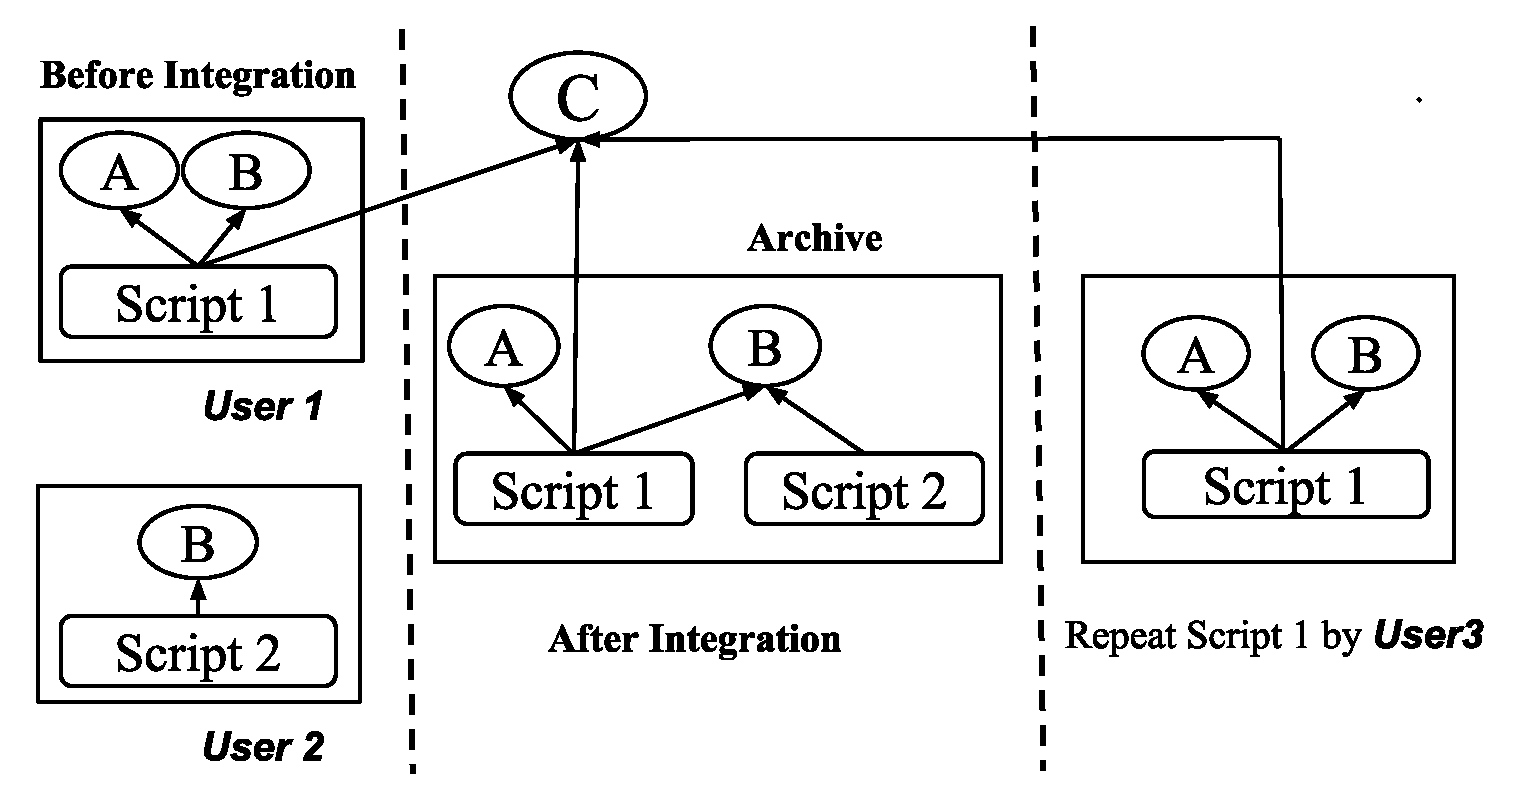
\epsfig{file=preservation-integration.eps, height=2.2in, width=3.3in}
\caption{Preservation Integration of Multiple Programs}
\label{fig:Preservation integration}
\end{figure}

To integrate the data and software from multiple analysis programs into one
package, the concrete information of data and software, such as size, version,
source and the number of files, need to be recorded. we also need to design one
more instructive shell script format, in which the data dependencies and
software dependencies can be clearly expressed and recognized. The packaging
process needs to be re-organized. Packaging utility needs to maintain one list
of current software and data subset already stored in the package. When one
user fork the packaging utility to preserve one program, the
packaging utility will scan the script, get the data and software dependency
part, judge whether each dependency has been inside the package, and only add
the new data and software into the package, and update the package information
and relavant retrieval information.

The architecture of preservation integration of multiple programs is shown in
Figure~\ref{fig:Preservation integration}. Script 1 and Script 2, sharing one
dependency B, belongs two different programs. Without preservation
integration, B will be preserved twice in the archive, which is
space-consuming. To improve the utilization efficiency of storage resources,
preservation integration of multiple programs is necessary. In the archive,
only one copy of B is stored, which is referred by both scripts and script 2.

\subsection{Preservation Granularity}

Another important factor of data and software preservation is the choice of
preservation granularity. In Solution 4, the preservation granularity is one
file, because Parrot virtual filesystem traps each system call and redirects
the access path of each file. As a result, during the packaging process, each
time only one file can be copied into the target package, which is
low-efficient. However, there are other options of preservation granularity.
The software is generally preserved in the unit of package inside the remote
repository, the packaging process of one experiment can adopt one package as
the unit. In addition, if the size of one whole software repository is small
and the access frequency of each package inside it is high, the granularity can
be set to the whole repository.

\subsection{Preservation of Large Data}

The preservation policy must concern about the size of data. If its size is
small, copying it into one pacakge and transferring it between different
machines is not a bad idea. Howerver, when the size becomes large, copying it
into one package will make the size of the package uncontrollable. In
Figure~\ref{fig:Preservation integration}, the size of C is very large and
easily to be obtained through Internet by different users. Directly referring C
as networked resources is more efficient than preserving it into one package.

\subsection{Mining of Dependencies} 

The mining degree of data and software dependencies greatly determines the
repeatability of one experiment. Data dependencies is easy to figured out. However, the situation of software dependencies is complex. The software
dependencies include OS, hardware platform, 
direct software dependencies and indirect software dependency which is dependent upon direct software dependencies.
The first
three categories are easy to deal with. The description of indirect software
dependencies needs more efforts. One solution is to utlize package management
tools, like rpm, pacman, apt, to recursively trace each direct software
dependency and generate one clear dependency graph. With the dependency graph,
the new user can configure the software environment and repeat the experiment.
Solution 4 odopts this solution, which is easy to implement, but leaves the
complex environment configuration to the new users. 

Another solution is to treat the computing environment, software environment
and scientific data as one integral entirety and preserve the entirety
completely. The reproduction of one experiment using this solution is easier.
However, the original machine is not only for one special experiment and may
concern a large amount of software and data unrelevant to the experiment. The
time and space overhead of this solution must be considered.

%\subsection{The preservation} When the authors and the programs becomes more
%and more, the whole pool of one repo may be nearly to be preserved. why not
%directly copy the whole repo and preserve it at the begining directly?  Answer:
%we must concern the efficiency of repeating one small and simple program.
\subsection{Preservation Degree of Directory Structure}

Data and software preservation of physics experiments must concern the
preservation degree of the original filesystem.  The three core components of
one filesytem are file, directory and metadata.  The access of files can be
divided into two categories: only access file metadata, like size, ownership,
access authority list, and access both the file content and metadata.  If both
the content and metadata need to be accessed, the whole file must be copies
into the package.  However, if only the metadata of one file is accessed, how
to preserve the file needs to be considered carefully. If the file size
is 1KB or 1MB, preserving the content is acceptable. If the size of one file is
1GB, preserving the whole file just for accessing its metadata is
inefficient.  

Directory is one list of files and subdirectories under it. At first, we only
copied the accessed items under one directory and ignored the unaccessed items.
However, some operations on one directory depends on each item under it. For
example, {\tt ls /dirA} is one linux command to list the name of each item under
{\tt /dirA}. Because the directory itself has the name list of items under it, only
the path of the directory was recorded into the namelist in the first phrase of
Solution 4. However, when we repeated the command {\tt ls /dirA} using the preserved package, it returned NULL because none of items under it existed in
value of {\tt ls /dirA}, the behavior of the whole program will become incorrect
and unpredictable. 

To ensure the semantics of the original program, all the items under one directory must be copied
into the package. However, the
time and space overhead appears again. Currently, Solution 4 creates one item
with the same name but the size of zero for each item under {\tt /dirA}. Another
solution is to introduce one database to preserve the metadata of each file and
directory. 

\subsection{User Access Model of Data and Software}

Through this case study, we noticed that the user access module of remote data
and software has a great impact of the preservation mechanism, especially when
we try to integrate the preservation of multiple programs. If all the programs
only refer the original data and software and refuse to modify them, the
preservation is easy and can ignore the data version problem. However, if some
programs try to modify the original data and software to accustom to its own
requirement, the preservation mechanism must provide one way to differentiate
the original data and the special data used in one certain
program. To have a clear understanding of the data access model, more examples
need to be investigated.

\subsection{Here is the Useful Package}

At the beginnig of our case study, we generated one package for Matthias's
example based on Solution 4. Several months later, the original machine meets
some problems and the access model of CMSSW was also modified. In this case, if
you want to repeat Matthias's example on the original machine, different 
configurations, including CMSSW\_ARCH, environment variables and CVS access
authority need to be modified. However, with the generated package and its map file, we can repeat the experiment directly on the same machine without any modification.
%here is the new content-hmeng

\section{Related Work }
\subsection{Software Preservation Approaches}

Generally, there are three approaches to preserve software environment:
technical/hardware preservation, migration and emulation.  Hardware
preservation preserves the original software and its original operating
environment. \cite{cifuentes1996binary} presented techniques used to migrate
legacy software running on register-based machines to modern RISC machines. \cite{mancl2001refactoring}
utilized one method called refactoring to make software migration become
easier. However, migration often involves the re-compiling and re-configuring
the source code to accustom a new hardware platform and software environment.
Emulation recreate the original software and hardware environment by
programming future platforms and OSs. One common solution to implement this is
virtual machine. According to the usage and emulation degree of the real
machine, virtual machine can be divided into system virtual machine and process
virtual machine. \cite{goldberg1974survey}\cite{smith2005architecture} introduced the working principle, design principle and
performance evaluation of system virtual machine. \cite{barham2003xen}\cite{kivity2007kvm}\cite{rosenblum1999vmware} illustrated the
functionality of  system VM to support different guest operating systems. \cite{esquembre2004easy} illustrated how JVM, one process virtual machine, can expedite the creation of
scientific simulations in Java. \cite{matthews2009towards}\cite{phelps2005no}\cite{hong2010software} discussed the pros and cons of each
approach.

\subsection{Software Environment vs Computing Environment}

\cite{matthews2009towards}\cite{phelps2005no}\cite{hong2010software} treated the preservation of computing environment and software environment as one entirety. However, frequently changing experiment software makes the maintenance of the preserved experimental environment very complex. 

\cite{buncic2010cernvm} treated them as two different categories. The preservation of computing environment is implemented with CernVM, and the preservation of software environment is based on a CernVM filesystem(CVMFS) specifically designed for efficient software distribution.

\subsection{Software Preservation Format}

\cite{zabolitzky2002preserving}\cite{castagne2013consider} emphasized the importance of preserving software in source code format. 

\cite{buncic2010cernvm} published pre-built and configured experiment software releases to avoid repeating the time-consuming software building procedure. 

\subsection{facilitate the reproduction of scientific experiments}

Attempts from different perspectives to facilitate the reproduction of scientific experiments utilizing preserved software library has been made. 
\cite{compostella2010cdf} discussed software distribution mechanism over the Grid using Parrot. 
\cite{blomer2011cernvm} proposed CVMFS to facilitate the software distribution over the network to CernVM. 
\cite{rice1996scientific} made the reproduction process easier through the integration of user interface, scientific software libraries, knowledge base into problem-solving environment.
\cite{kohn2001divorcing} tried to enable the creation and distribution of language-independent software library by addressing language interoperability.

\subsection{figure out the absolutely relevant data and software }

Current mechanisms of preserving scientific experiments assume that all the data and software mentioned in the experiments are necessary for the reproduction of the experiments. However, this is not always right. In some cases, the original author may leave additional code referring to irrelative data and software in the experiment programs. One mechanism, which can figure out the absolutely relevant data and software of one experiment, is important for both the preservation and reproduction of scientific experiments.

\subsection{the importance of case study}
\cite{matthews2008significant} introduced one conceptual framework for software preservation from several case studies of software preservation
\cite{matthews2010framework} designed a tool to capture software preservation properties within a software environment through a series of case studies conducted to evaluate the software preservation framework.
\cite{johnston2014workflow} proposed one overall data curation workflow for 3-5 case studies of preserving research data.
To figure out how to preserve HEP applications, this paper studies one case of preserving one representative HEP application.


\section{Conclusion}


\bibliographystyle{abbrv}
\bibliography{cclpapers,this}

\end{document}
